\section{Traitement des données et formats de fichiers}

TECHNI DRONE utilise plusieurs logiciels pour le traitement des donnéées après
les campagnes d'acquisition faites par drones. Cette etape est tres importante 
dans la mesure ou elle aboutie à la realisation des carte representant une carriere.

\begin{figure}[h]
  \begin{minipage}[c]{.46\linewidth}
      \centering
      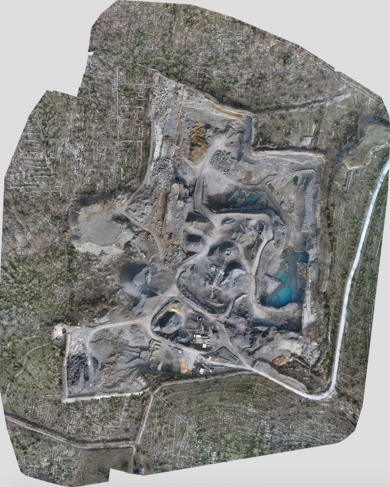
\includegraphics[width=8cm, height=8cm]{images/orthomosaique.png}
  \end{minipage}
  \hfill%
  \begin{minipage}[c]{.46\linewidth}
      \centering
      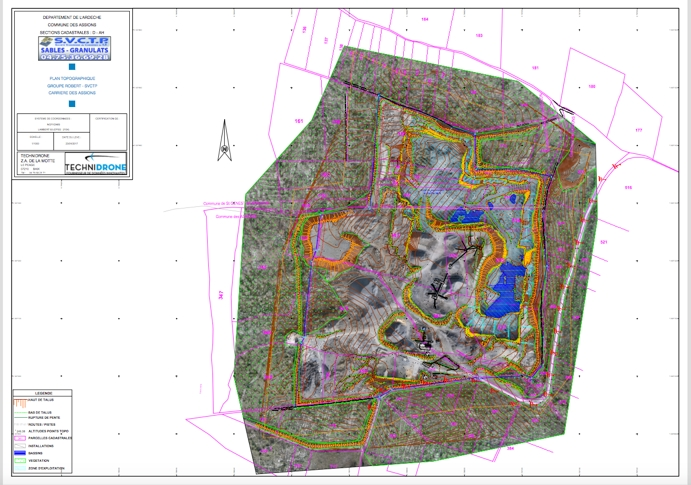
\includegraphics[width=8cm,height=8cm]{images/carteCarriere.jpg}
  \end{minipage}
  \caption{L’ortho mosaïque de la carrière et la carte de la carrière.
     \label{fig:credit}}
\end{figure}

\subsection{Pix4D}

Le traitement des images acquisent par drones est fait avec le logiciel Pix4D.
Pix4D est un logiciel de photogrammétrie pour la cartographie professionnelle 
basée sur des images de drones uniquement. 
\begin{figure}[h]
  \begin{center}
    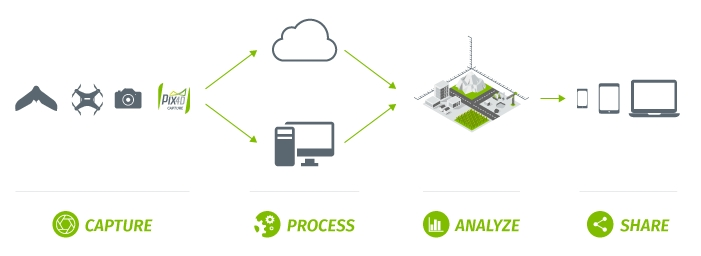
\includegraphics[width=12cm]{images/processusPix4D.jpg}
     \caption{Processus de traitement Pix4D.
     \label{ProcesPix4D}}
  \end{center}
\end{figure}
Le logiciel convertit les images 
aeriennes prise par drones en orthomosaiques 2D georeferencées, en model 
surface 3D texturé et en nuages de points. ce processus prend environ une dizaine
d'heures comment le montre la Figure~\ref{ProcesPix4D}. 

Dans la Figure~\ref{positionImage}, les points rouges representent les positions
des images prises drone et Les croix bleues sont les points GCPs
(Group Control Point)\footnote{Les GPCs sont des 
marqueurs visuels sur le sol avec des coordonnées connues qui augmentent 
la précision ortho mosaïque et permettent l'alignement de plusieurs 
campagnes d’acquisition.}. Le logiciel utilise les coordonnées des ces point
pour faire le recalage des images et produit les nuages de point et le maillage 3D
de la carrière. Le logiciel met aussi à disposition des outiles pour la detection
manuel des ligne de ruptures de pente directement sur les nuages de points ou
sur le maillage 3D. Les coordonnées de ces ligne ainsi detecter sont enregistrer
dans un fichier au format shapefile(.shp)\footnote{Shapefile est un format
de fichier ouvert compatible avec le logiciel OpenSource QGIS}. Cette phase
d'annotation prend egalement une dizaine d'heure pour un employé habitué au logiciel.
La Figure~\ref{annotationMallage} montre triangulaire 3D créé par pix4D,
sur lequel se basé pour détecter les lignes de ruptures de pente.

\begin{figure}[h]
  \begin{center}
    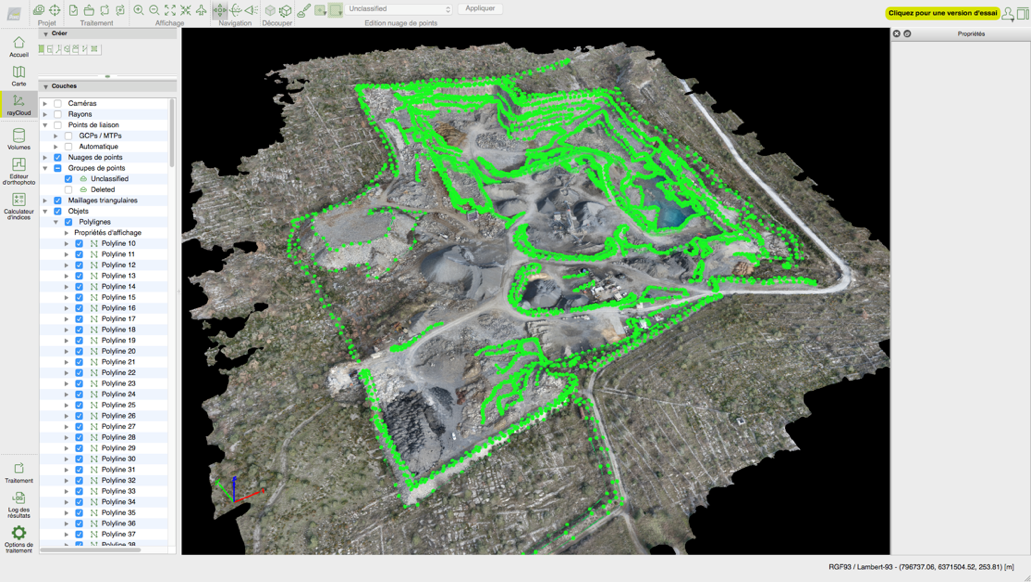
\includegraphics[width=12cm, height=5cm]{images/detctionLigne.jpg}
     \caption{Detection manuel des lignes de ruptures de pente.
     \label{detctionLigne}}
  \end{center}
\end{figure}
\begin{figure}[h]
  \begin{center}
    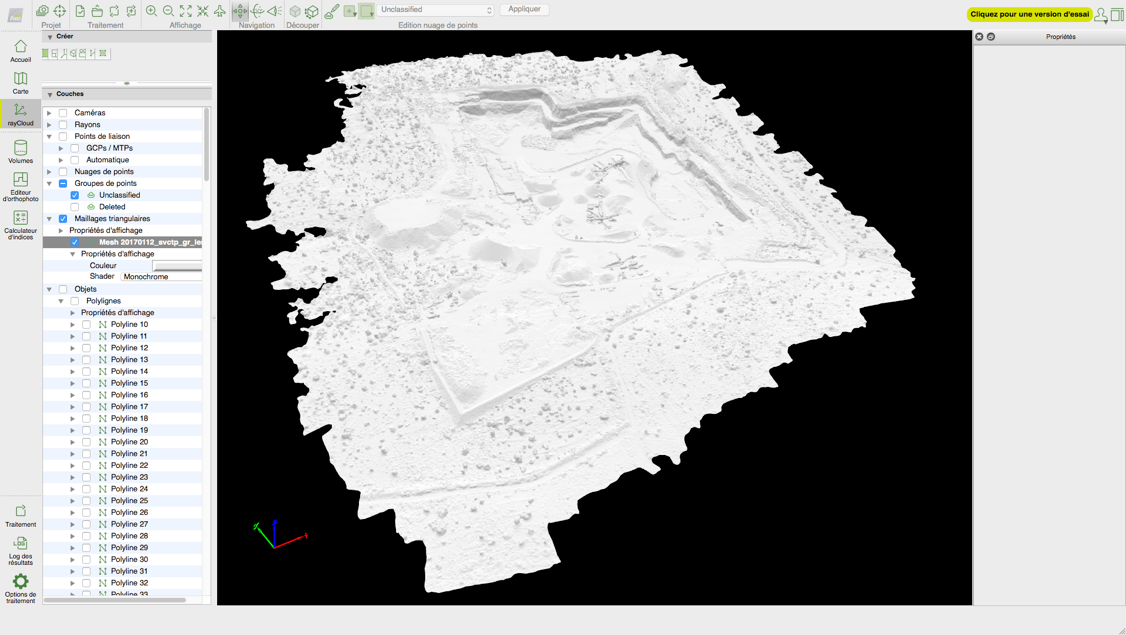
\includegraphics[width=12cm,height=5cm]{images/maillageSansTexture.jpg}
     \caption{Maillage 3D sans texture.
     \label{maillageSansTexture}}
  \end{center}
\end{figure}
\begin{figure}[h]
  \begin{center}
    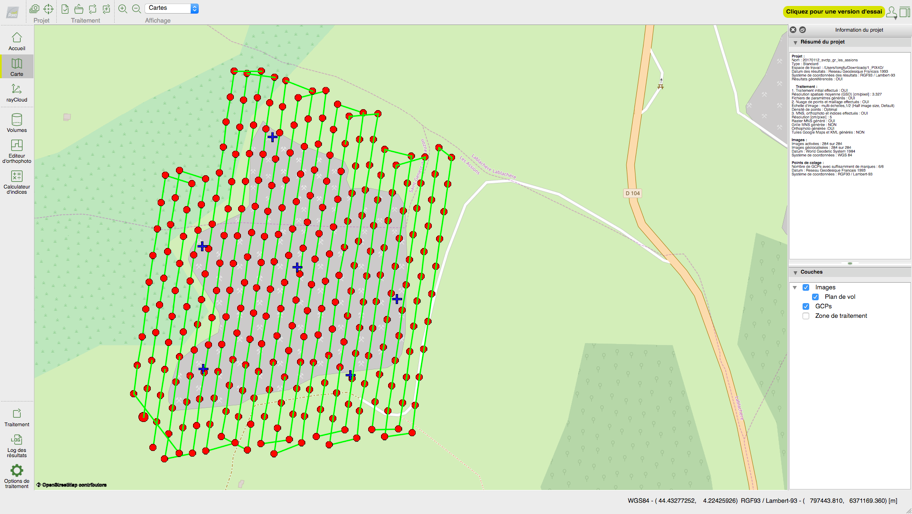
\includegraphics[width=12cm]{images/positionImagePix4D.jpg}
     \caption{Position des images prise par drones.
     \label{positionImage}}
  \end{center}
\end{figure}

\subsection{QGIS}

QGIS est un logiciel SIG (système d'information 
géographique) libre multiplate-forme publié sous licence GPL. 
il gère les formats d’image matricielles (raster) et vectorielles,
ainsi que les bases de données [Wikipedia](https://en.wikipedia.org/wiki/)\dots
TECHNI-DRONE utilise ce logiciel pour classifier les lignes de 
ruptures de pente par rapport aux courbes de niveau.
\begin{figure}[h]
  \begin{center}
    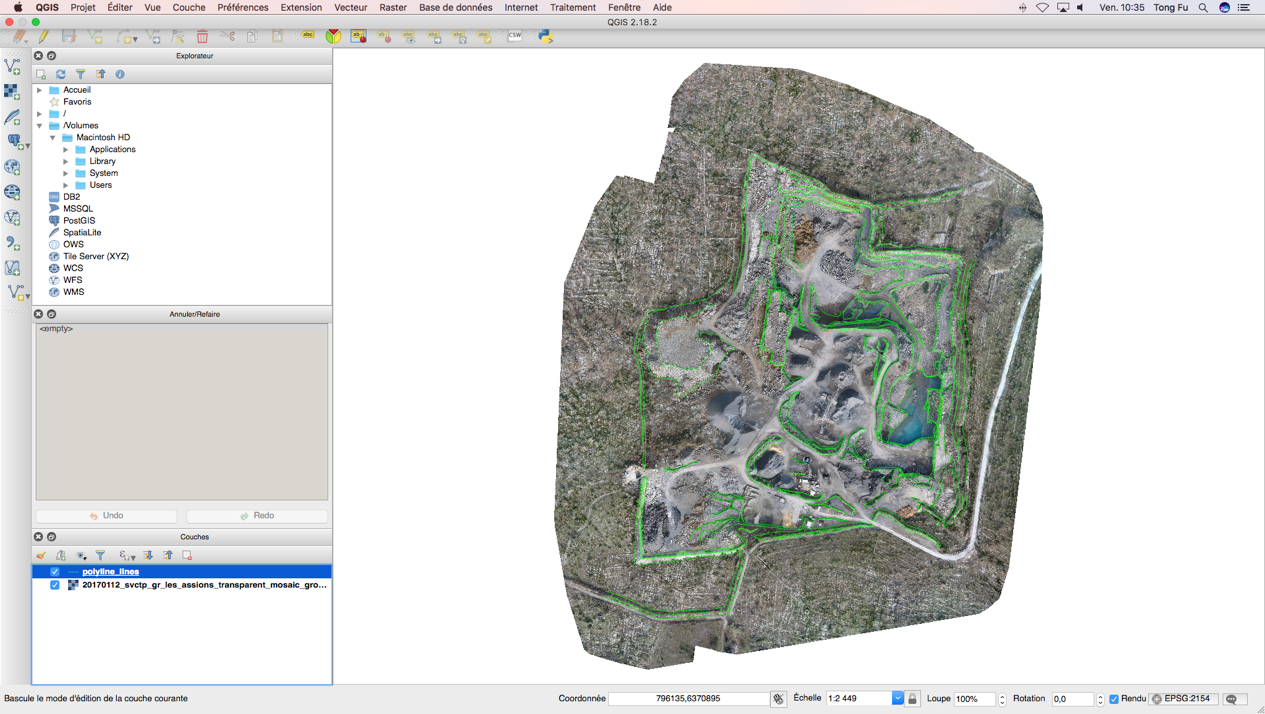
\includegraphics[width=12cm]{images/QGIS.jpg}
     \caption{Classification sur QGIS.
     \label{QGISClassification}}
  \end{center}
\end{figure}
